\documentclass[a4paper,dvipsnames, 11pt]{article}
\usepackage{latexsym}
\usepackage{amsmath}
%\usepackage{mathspec}
%\usepackage{amsthm}
% \usepackage{amssymb}
% \usepackage{textcomp} 
% \usepackage{ulem}
% % \usepackage{fontspec}     
\usepackage[british]{babel}
\usepackage{enumitem}
% \usepackage{pifont}
\usepackage[a4paper, margin=1.2in]{geometry}
\usepackage{hyperref}
\usepackage[dvipsnames, table]{xcolor}
\usepackage{tikz}
% \usepackage{mathrsfs}

% \usepackage{eucal}
\usepackage{dsfont}
% \usepackage[most]{tcolorbox}
% \usepackage{mathdots}
\usepackage{minted} %? used for code-integration
% \usepackage{titling}
\usepackage[bibitemsep=100pt, citestyle=alphabetic,bibstyle=alphabetic]{biblatex}

\definecolor{darkmagenta}{RGB}{99,0,99}
\hypersetup{
    colorlinks,
    citecolor=darkmagenta,
    filecolor=darkmagenta,
    linkcolor=darkmagenta,
    urlcolor=darkmagenta
} %? Change hyperlink's styles

%%%%%%%%%%%%%%? courbes
\usepackage{amsfonts,amscd}
\usepackage{pgfplots}
%%%%%%%%%%%%%?

%%%%%%%%%%%%%
\DeclareMathOperator{\mat}{Mat}
\DeclareMathOperator{\card}{Card}
\DeclareMathOperator{\len}{len}
\DeclareMathOperator{\erf}{erf}
%%%%%%%%%%%%%


%%%%%%%%%%%%%
\newcommand{\dt}{\mathrm{d}}
\newcommand{\un}{\mathds1}
\renewcommand{\o}{\scriptstyle\mathcal{O}}
\renewcommand{\O}{\mathcal{O}}
\renewcommand{\emptyset}{\varnothing}
\newcommand{\lbd}{\lambda}
\renewcommand{\phi}{\varphi}
\def\inte #1 #2 { [\![#1,#2]\!] }
%%%%%%%%%%%%%


%%%%%%%%%%%%%
\newcommand{\N}{\mathbb{N}}
\newcommand{\R}{\mathbb{R}}
\newcommand{\Z}{\mathbb{Z}}
\newcommand{\C}{\mathbb{C}}
\newcommand{\K}{\mathbb{K}}
\newcommand{\Q}{\mathbb{Q}}
\renewcommand{\P}{\mathbb{P}}
\newcommand{\M}{\mathcal{M}}
\renewcommand{\r}{\mathcal{R}}
\renewcommand{\S}{\mathcal{S}}
%%%%%%%%%%%%%


\renewcommand{\arraystretch}{1.4} %? For better matrix
\renewcommand{\thesection}{\arabic{section}} %? Roman number for sections


\newenvironment{code}{
    \VerbatimEnvironment
    \begin{minted}[mathescape,
        linenos,
        numbersep=5pt,
        gobble=2,
        frame=lines,
        framesep=2mm]{cpp}%
}{
        \end{minted}%
}

    \setcounter{secnumdepth}{4}
    \setcounter{tocdepth}{4}

\hbadness=10000
\vbadness=10000
\flushbottom
\addbibresource{rapport.bib}
\usepackage{tkz-base}
\usepackage{algorithm}
\usepackage{algorithmic}
\usepackage{wrapfig}
\usepackage{subcaption}
\usepackage{changepage}
\usepackage[]{tocbibind}
\usepackage[useregional]{datetime2}
\usepackage{adjustbox}
\usepackage{pdfpages}
\usepackage{tabularx}
\usepackage{array}
\usepackage{cleveref}
\usepackage{multicol}
\usepackage{graphicx}
\usepackage{multirow}
\usepackage[multiple]{footmisc}
\usepackage[minNoteWidth=1cm,
    colorinlistoftodos,
    backgroundcolor=magenta!30!white,
    bordercolor=magenta]{luatodonotes}
\usepackage{amssymb}

\newcolumntype{C}{>{\centering\arraybackslash}X}
\newcolumntype{s}{>{\hsize=.3\hsize\linewidth=\hsize}C}
\newcolumntype{D}{>{\hsize=.4\hsize\linewidth=\hsize}C} %Double width column

% \setlength{\bibhang}{0pt}

% \defbibenvironment{bibliography}
% {\list{\printtext[labelalphawidth]{\printfield{labelprefix}\printfield{labelalpha}}}% Updated line
% {\setlength{\labelwidth}{\labelalphawidth}% Updated line
% \setlength{\leftmargin}{0pt}%
% \setlength{\labelsep}{\biblabelsep}%
% \setlength{\itemsep}{\bibitemsep}%
% \setlength{\itemsep}{0pt}% Set to 0pt to remove vertical space
% \setlength{\parsep}{\bibparsep}}%
% \renewcommand*{\makelabel}[1]{\hss\hspace{\dimexpr\labelalphawidth+\labelsep}##1}}
% {\endlist}
% {\item}

% Redefine the footnotetext command to remove indentation
\makeatletter
\renewcommand\@makefntext[1]{%
    \noindent\makebox[0em][r]{\@thefnmark\hspace{5pt}}#1}
\makeatother

\newcommand{\reftodo}[1][]{\todo[backgroundcolor=green!30!white, bordercolor=green, #1]{\thesubsubsection{}~Ref} {\color{red} REF}}
\newcommand{\missingtext}[1][]{\todo[inline, caption=\thesubsection~Fill missing text, backgroundcolor=cyan!30!white, bordercolor=cyan]{#1}}
%\usepackage[]{todonotes}

\setlength\parindent{0pt}

\usetikzlibrary{shapes.multipart}

\makeatletter
\newenvironment{fixedfigure}
{\def\@captype{figure}\center}
{\endcenter}
\makeatother



% \usepackage{graphicx,txfonts}

\addto\captionsbritish{
    \renewcommand{\contentsname}%
    {Table of content}%
}

\renewcommand{\today}{\number\day\textsuperscript{\scriptsize\text{th}} \DTMenglishmonthname{\month} \number\year}


\makeatletter
\newcommand\setxveclength[5]{% newmacro, node1, node2
    \pgfpointdiff{#2}{#3}
    \edef#1{\the\pgf@x}
}
\makeatother

\sloppy                  

\pgfplotsset{compat=1.16}

\begin{document}


%\setmathfont{Latin Modern Math}
%\setmathfont[range={\mathscr,\mathbfscr}]{XITS Math}

% \maketitle



\begin{titlepage}
    \begin{center}
        \vspace*{1cm}
            
        \Huge
        \textbf{Random Osborne Algorithm for Matrix Balancing}
            
        \vspace{0.5cm}
        \LARGE
        Optimal transport report
            
        \vspace{2.5cm}
            
        \huge {\sc Alexi Canesse\footnote{\href{mailto:alexi.canesse@ens-lyon.fr}{alexi.canesse@ens-lyon.fr}, ENS de Lyon, France}\footnote{\href{mailto:alexi.canesse@ens-paris-saclay.fr}{alexi.canesse@ens-paris-saclay.fr}, ENS Paris-Saclay, France}}\\\Large
            
        \vfill

        Optimal transport course\\
        Part of the MVA program at ENS Paris-Saclay.
            
        \vspace{2cm}
        
\includegraphics[width=0.5\textwidth]{./figures/logo.pdf}
        \vspace{2cm}

        \Large
        Computer Science and Mathematics\\
        École Normale Supérieur Paris-Saclay\\
        École Normale Supérieur de Lyon\\
        Paris, France\\
        \today
            
    \end{center}
\end{titlepage}





\newpage

%\tableofcontents
\makeatletter
\section*{Table of content}
\vspace{.05\textwidth}
\@starttoc{toc}
\thispagestyle{empty} % Remove page number from the ToC page
\clearpage % Start the new page without page number

\setcounter{page}{1} % Reset page counter and set page number to 1

\makeatother
\newpage

\vspace*{10pt}
\todo[inline, caption={Abstract}]{Abstract (½ page): 
    What problems is studied? 
    Why is it relevant? 
    What solutions is proposed? 
    Which contributions (theory, numerics, etc)? }
% \begin{adjustwidth}{30pt}{30pt}
%     \textit{
%         Accurate physics simulations can be computationally expensive due to the requirement of fine meshes.
%         However, a cost-effective approach involves reducing the mesh size while retaining crucial features required
%         for the simulation.
%         Some of these features are conveniently represented in the spectra of Laplacians operators defined on the mesh.
%         There exists a coarsening method that filters out unnecessary spectral bands.
%         The challenge lies in determining which spectral bands are important for the simulation, as \textbf{this information is
%         largely unknown}.
%     }\\

%     \textit{
%         To address this, we propose a \textbf{novel approach} to guide the coarsening process using \textbf{insights
%         from physical simulations}.
%         By learning the spectral subspaces that significantly influence the simulation outcomes, we can create a coarse
%         mesh that retains the characteristics essential for an accurate simulation.
%         Main contributions are:
%         \begin{itemize}
%             \item A novel spectral optimization method for coarsening, with physical simulations in mind.
%             \item Understanding importance of spectral subspaces: By understanding the spectral subspaces that contribute
%             the most to the simulations, we gain valuable insights into the underlying physics and behavior of the system.
%             \item Faster simulation times: The reduced mesh size leads to a considerable speed-up in the simulation
%             process, making it more efficient and feasible for practical applications.
%         \end{itemize}
%     }
% \end{adjustwidth}
\vspace*{10pt}

\section{Introduction (3 pages)}

\cite{altschuler2023near}

\subsection{Presentation of the problem}

The matrix balancing problem arises from the recognition that matrices encountered in practical applications may have varying scales across rows and columns. These imbalances can lead to numerical instability and adversely impact the accuracy of numerical computations such as eigenvalues/eigenvectors decomposition~\cite{chen2000balancing, chen2001preconditioning} or solving linear systems~\cite{chen2001preconditioning}, . Matrix balancing algorithms aim to address these issues by adjusting the scaling of rows and columns, thereby enhancing the overall numerical properties of the matrix.\\

Other problems can be reduced to matrix balancing, which gives direct applications. For instance, in optimal transport with problems where decision variables are probability distributions~\cite{altschuler2022transport}; the approximating Min-Mean-Cycle which can be solved in near-linear runtime in the number of edges~\cite{altschuler2022approximating} using results from matrix balancing and in particular, the main result of the studied article. 

\nota{Let \(c\) and \(r\) respectively be the column-wise sum and the row-wise sum of matrices \textit{ie.}
\[
    c : \left\{\begin{array}{rcl}
        \M_{n,m}(\K) & \to &\K\\
        A & \mapsto &  A^\top \mathbf{1}
    \end{array}\right. \quad \text{and} \quad r: \left\{\begin{array}{rcl}
        \M_{n,m}(\K) & \to &\K\\
        A & \mapsto & A \mathbf{1}.
    \end{array}\right.
\]}

\defn{Let \(A \in \M_n(\R_+)\) be a non negative square matrix, \(\varepsilon \geq 0\) and \(k \in \N^\star\). The matrix \(A\) is \((\varepsilon, k\)\)-balanced if 
\begin{align}\label{norm}
    \dfrac{||c(A) - r(A)||_k}{\sum_{i,j} a_{i,j}} \leq 0.
\end{align}
Furthermore, if \(A\) is \((0, k)\)-balanced, we say that \(A\) is balanced.}

\defn{The \(\varepsilon, k\)-\textbf{approximate matrix balancing problem} is: given a square non-negative matrix \(K \in \M_n(\R_+)\), \(\varepsilon \geq 0\) and \(k \in \N^\star\), find a vector \(x \in \R^n\) such that \(\mathcal D(e^x)K\mathcal D(e^{x})\) is \((\varepsilon, k)\)-balanced.}

\subsection{Related work}

\paragraph*{Iterative algorithms} The \txtsc{Osborn} algorithm, introduced by \textsc{Osborn} in \cite{osborne1960pre} and later discussed in~\cite{parlett1971balancing}, is implemented in Scipy as a default matrix balancing method. Other iterative methods have been introduces. Notably, the \textsc{Sinkhorn-Knopp} algorithm~\cite{sinkhorn1967concerning}, a special case of \textsc{Bregman}’s balancing method~\cite{lamond1981bregman}, iteratively rescales each row and column until convergence. However, it converges linearly, which is impractical for large and sparse matrices, as discussed by \textsc{Soules} et al. in~\cite{soules1991rate}. \textsc{Parlett} introduced an approach in~\cite{parlett1971balancing} to approximately balance matrices by ensuring the diagonal consists only of powers of 2. The advantage of this method is the elimination of floating-point errors when computing the balanced matrix on base-two computers, making it ``good enough'' in practice. Some efforts are also made to compare balancing algorithms on real use cases~\cite{schneider1990comparative}.

\paragraph*{Issues in Matrix Balancing} While matrix balancing is generally effective, there are corner cases where it can worsen the conditioning of matrices. \textsc{Watkins} et al. highlighted some of these cases in~\cite{watkins2006case}. Additionally, \textsc{James} et al. explained, in~\cite{james2014matrix}, these issues and proposed modifications to LAPACK to mitigate them.

\paragraph*{Theoretical bounds}  \cite{kalantari1996complexity} establishes an upper bound on the norm of the scaling factors and presents a polynomial-time complexity bound for the computation of scaling factors with a prescribed accuracy.

\paragraph*{Characterizations of Non-Negative Balancable Matrices} \cite{osborne1960pre} and \cite{eaves1985line} offer characterizations of non-negative balancable matrices, contributing to the theoretical understanding of the properties of such matrices. Additionally, \cite{kalantari1997complexity} provides insights into the complexity aspects of this problem.

\paragraph*{Tensor Matrix Balancing} \textsc{Sugiyama} et al. extended matrix balancing to tensors in~\cite{sugiyama2017tensor}, providing a perspective on balancing operations in multi-dimensional spaces. This work contributes to the broader understanding of matrix balancing techniques applied beyond traditional matrices.

\subsection{Contributions of the paper}

Their main contribution is \Cref{main_thm}. It exhibits a variant of \textsc{Osborn}'s algorithm with near-linear runtime in the input sparsity. It also shows that improving the runtime dependence in \(\varepsilon\) can be improve from \(\varepsilon^{-2}\) to \(\varepsilon^{-1}\) without an additional factor \(n\).  

\thm{\label{main_thm}Let \(K \in \M_n(\R_+)\) be a balanceable non negative square matrix and \(\varepsilon \geq 0\). Random \textsc{Osborn} solves \((\varepsilon, 1)\)-approximate matrix balancing problem in \(T\) operations where there exists \(c > 0, \delta > 0\) such that 
\[
    \mathbb E(T) = \mathcal O \left(\dfrac{m}{\varepsilon}\min\left\{\dfrac{1}{\varepsilon}; d\right\} \log \kappa\right)  \quad \text{and} \quad \mathbb P \left(T \leq c \dfrac{m}{\varepsilon}\min\left\{\dfrac{1}{\varepsilon}; d\right\} \log \kappa \log \dfrac{1}{\delta}\right) \geq 1 - \delta
\]
where \(m\) is the number of nonzero entries in \(K\), \(d\) is the diameter of the graph associated to \(K\) and \(\kappa = \sum_{i,j}K_{i,j}/\min_{i,j}{K_{i,j}}\).}

\subsection{Our contributions}

numerics?
limits? 
optimization ?

\section{Main body (10 pages)}

\subsection{Notations}

\subsection{Presentation of the method}


\begin{code}
osborn(|\(K\)|, |\(\varepsilon\)|):
    x = 0 |\(\in \R^n\)|
    while not(is_balanced(|\(\D(e^x) K \D(e^{-x})\)|, |\(\varepsilon\)|)):
        Choose k |\(\in\)| [n] # This is where variants differ
        x += (log(c_k(|\(\D(e^x) K \D(e^{-x})\)|)) - log(r_k(|\(\D(e^x) K \D(e^{-x})\)|)))/2
    return x
\end{code}

There are \textit{many} way to choose the next coordinate to update and hence many variants of the algorithm. The article focuses on four of them:
\begin{itemize}
    \item \textbf{Cyclic \textsc{Osborn}} Cycle through the coordinates. (\textit{eg.} {\color{magenta}1, 2, 3}, {\color{cyan}1, 2, 3}, {\color{red}1,} \dots).
    \item \textbf{Random-Reshuffle Cyclic \textsc{Osborn}} Cycle through the coordinates using a new random permutation for each cycle. (\textit{eg.} {\color{magenta}2, 1, 3}, {\color{cyan}1, 2, 3}, {\color{red}1, 3, 2}, \dots).
    \item \textbf{Greedy \textsc{Osborn}} Choose \(k\) where the imbalance is maximal \textit{eg.}
    \[
        k = \argmax_{k}\left|\sqrt{r_k(\D(e^x) K \D(e^{-x}))} - \sqrt{c_k(\D(e^x) K \D(e^{-x}))}\right|.    
    \]
    \item \textbf{Random \textsc{Osborn}} Uniformly sample \(k\) independently between each call.
\end{itemize}

\subsubsection{Implementation}

The implementations were carried out in Python, providing us with a transparent and customizable framework for thorough experimentation. The source code for our implementations is available on \href{https://github.com/alexicanesse/Near-linear-convergence-of-the-Random-Osborne-algorithm-for-Matrix-Balancing}{GitHub}. The implementation uses sparse representation for matrices and aimed to provide an implementation using data structures as close as possible as those used to compute the theoretical results. However, we were not able to find a detailed presentation of those and had to do our best to match the article. We did not give any focus on bit complexity. The authors recommanded a log-domain implementation to enable a logarithmic bit-complexity for some variants. However, we decided not to follow through in order to increase speed because we did not worry about bit-complexity.\\

At each update of \(x\), we update the balanced matrix by multiplying the corresponding row and column. With the sparse representation, this operation is proportional to \(m\). It is even \(\mathcal O(m/n)\) on average! To compute the optimization function, the sum of elements in \(DAD^{-1}\) is computed in \(\mathcal O (m)\) thanks to the sparse representation and \(||c(A) - r(A)||_1\) is also computed in \(\mathcal O(m)\). Indeed, we use \(||c(A) - r(A)||_1 = \sum_j \left| \sum_i (DAD^{-1} - (DAD^{-1})^\top)_{i,j}\right|\). \textbf{Those techniques are not presented in the article and we had to come up with on our own.}\\

\subsection{Matrix balancing as a convex optimization problem}

A key part of the proofs of convergence given on the paper and other works rely mainly on a seeing the matrix balancing problem as an optimization problem. Let \(\Phi : x \mapsto \log \sum_{i,j} e^{x_i - x_j} K_{i,j}\). The gradient of this function is 
\[
    \nabla \Phi (x) = \dfrac{r\left( \mathcal D(e^x)K\mathcal D(e^{x}) \right) - c\left( \mathcal D(e^x)K\mathcal D(e^{x}) \right)}{\sum_{i,j}\left( \mathcal D(e^x)K\mathcal D(e^{x}) \right)_{i,j}}.    
\]

We can clearly notice a connection with \Cref{norm} and see that \(x\) is a solution to the \(\varepsilon, k\)-matrix balancing problem if and only if \(||\nabla \Phi(x)||_k \leq \varepsilon\). The function \(\Phi\) is convex and approximately solving the convex optimization problem \(\min_x \Phi(x)\) solves the matrix balancing problem.\\

Alexandre d'Aspremont says in his MVA course on convex optimization that writing a problem as a convex optimization problem is almost solving it, which shows how important this statement is.

\subsection{Theoretical guarantees}\label{theoritical}

\begin{lemma}\label{balanceability}
    A matrix \(K \in \mathcal M_n(\R_+^\star)\) is balanceable if and only if its associated graph is strongly connected~\cite{osborne1960pre}.
\end{lemma}

\thm{\label{greedy_thm}Let \(K \in \M_n(\R_+)\) be a balanceable non negative square matrix and \(\varepsilon \geq 0\). Greedy \textsc{Osborn} solves \((\varepsilon, 1)\)-approximate matrix balancing problem in 
\[
    \mathcal O \left(\dfrac{\color{magenta} n^2}{\varepsilon}\min\left\{\dfrac{1}{\varepsilon}; d\right\} \log \kappa\right) 
\]
where \(d\) is the diameter of the graph associated to \(K\) and \(\kappa = \sum_{i,j}K_{i,j}/\min_{i,j}{K_{i,j}}\).}

\thm{\label{main_thm}Let \(K \in \M_n(\R_+)\) be a balanceable non negative square matrix and \(\varepsilon \geq 0\). Random \textsc{Osborn} solves \((\varepsilon, 1)\)-approximate matrix balancing problem in \(T\) operations where there exists \(c > 0, \delta > 0\) such that 
\[
    \mathbb E(T) = \mathcal O \left(\dfrac{\color{magenta} m}{\varepsilon}\min\left\{\dfrac{1}{\varepsilon}; d\right\} \log \kappa\right)  \quad \text{and} \quad \mathbb P \left(T \leq c \dfrac{\color{magenta} m}{\varepsilon}\min\left\{\dfrac{1}{\varepsilon}; d\right\} \log \kappa \log \dfrac{1}{\delta}\right) \geq 1 - \delta
\]
where \(m\) is the number of nonzero entries in \(K\), \(d\) is the diameter of the graph associated to \(K\) and \(\kappa = \sum_{i,j}K_{i,j}/\min_{i,j}{K_{i,j}}\).}

\thm{\label{random_cyclic_thm}Let \(K \in \M_n(\R_+)\) be a balanceable non negative square matrix and \(\varepsilon \geq 0\). Random cyclic \textsc{Osborn} solves \((\varepsilon, 1)\)-approximate matrix balancing problem in \(T\) operations where there exists \(c > 0, \delta > 0\) such that 
\[
    \mathbb E(T) = \mathcal O \left(\dfrac{\color{magenta} mn}{\varepsilon}\min\left\{\dfrac{1}{\varepsilon}; d\right\} \log \kappa\right)  \quad \text{and} \quad \mathbb P \left(T \leq c \dfrac{\color{magenta} mn}{\varepsilon}\min\left\{\dfrac{1}{\varepsilon}; d\right\} \log \kappa \log \dfrac{1}{\delta}\right) \geq 1 - \delta
\]
where \(m\) is the number of nonzero entries in \(K\), \(d\) is the diameter of the graph associated to \(K\) and \(\kappa = \sum_{i,j}K_{i,j}/\min_{i,j}{K_{i,j}}\).}

\subsection{Numerics}

Computing numeric experiments was not easy. Getting the actual number of arithmetic operations is a complex endeavour, especially with a high-level language such as Python. We decided do use the running time to estimate how the number of arithmetic operations will evolve as a function of given parameters. This is not a precise measurement. However, all algorithms presented are are basically the same and this measure should be a fair assessment of convergence speed. 

\todo[inline, caption={numerics}]{it indeed converges even with high sparsity (cf theorem)\\

LOOK IN {schneider1990comparative} https://sci-hub.st/10.2307/171357 for inspiration on applications\\

per iteration runtime (1.3)}

\subsubsection{Data generation}\label{data_genaration}

In order to conduct numerical experiments, it is useful to be able to generate matrices with given parameters such as value of \(\kappa\) and sparsity. For that, we start by generating a \((n,n)\) random matrix with \(m\) non-zero values using \mintinline{python}{scipy.sparse.random}. Then we assign values to those non-zero entries according to a \textsc{exponential} distribution of scale 1. We then want to modify those values to get the expected value for \(\kappa\). To do so, we add a value \(x\) to all non-zeros entries. If the generated matrix was \(K\), to find \(x\), we solve 
\[
    \kappa = \dfrac{\sum_{i,j} K_{i,j} + m \times x}{K_{\text{min}} + x}.
\]        

We then find that the value to add is 
\[
    x = \dfrac{\kappa \times K_\text{min} - \sum_{i,j}K_{i,j}}{m - \kappa}.   
\]

Sometimes, \(x\) is negative and \(K\) end up not being non-negative and we just start again from the start. Finally, we want the matrix to be balanceable. Hence, we start again until its associated graph is strongly connected (\Cref{balanceability}). 

\subsubsection{Complexity as a function of \(n\)}

In order to experimentally show the convergence speed of theorems presented in~\Cref{theoritical}, we fixed the parameters \(m\) and \(\varepsilon\) and let \(n\) in \(\inte 20 60 \). Each matrix is generated using an exponential distribution according to the scheme\footnote{Note that here \(\kappa\) is not fixed.} presented in~\Cref{data_genaration}. The~\Cref{fig:n} shows the results.

\begin{figure}[H]
    \centering
    \begin{subfigure}[b]{.24\textwidth}
        \centering
        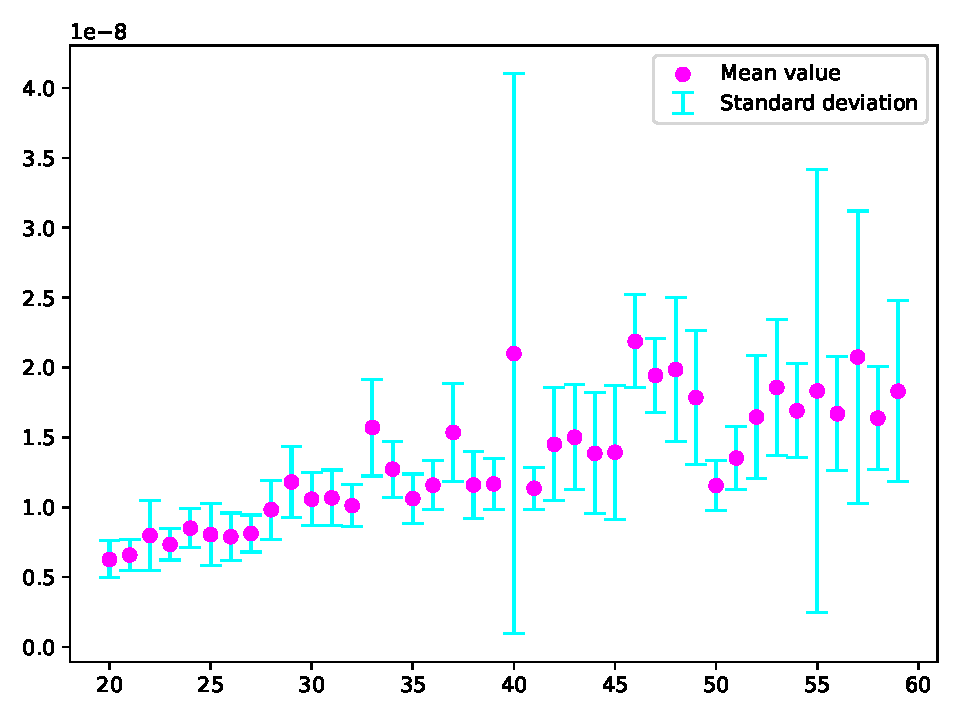
\includegraphics[width=\textwidth]{figures/n/random_function_of_n_n_20_60__kappa_55582.80548329922}
        \caption{Random.}\label{fig:na}
    \end{subfigure}
    \hfill
    \begin{subfigure}[b]{.24\textwidth}
        \centering
        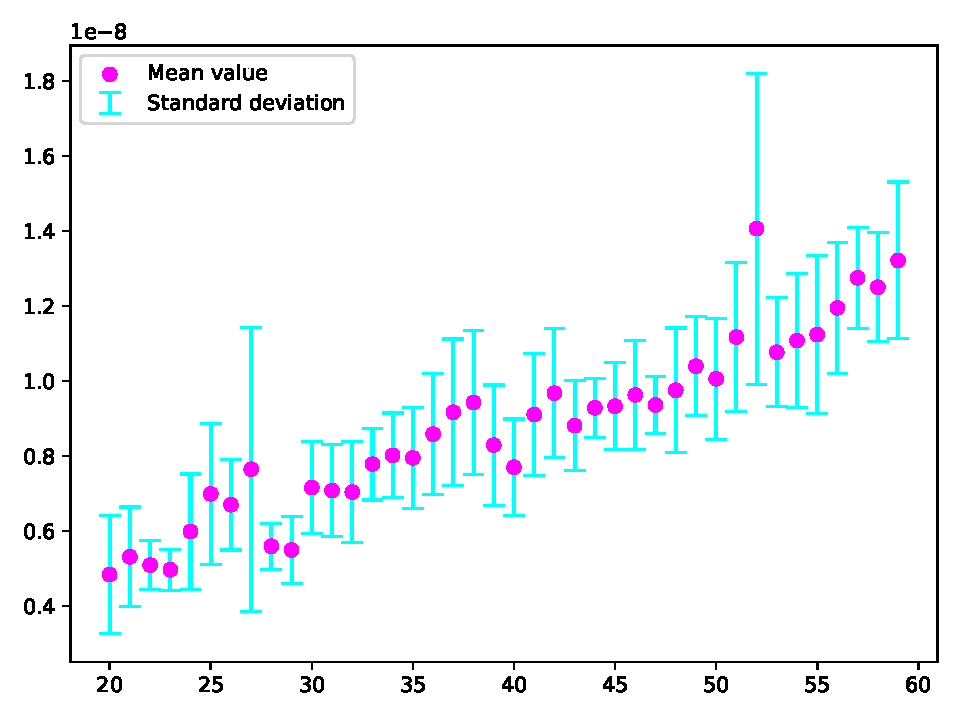
\includegraphics[width=\textwidth]{figures/n/random_cyclic_function_of_n_n_20_60__kappa_300}
        \caption{Random cyclic.}\label{fig:nb}
    \end{subfigure}
    \hfill
    \begin{subfigure}[b]{.24\textwidth}
        \centering
        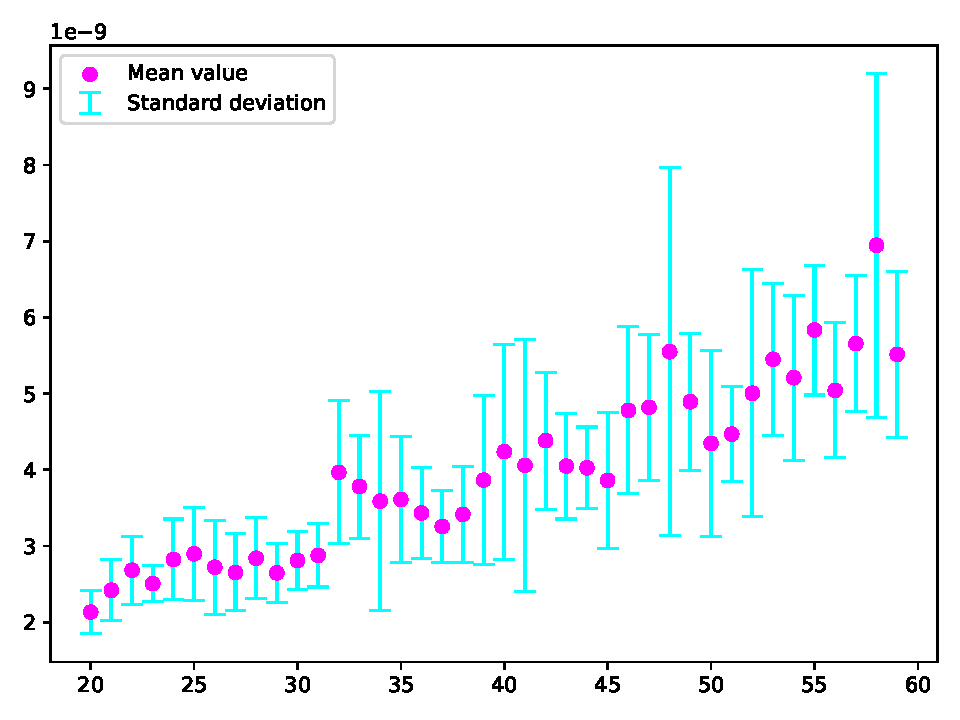
\includegraphics[width=\textwidth]{figures/n/greedy_function_of_n_n_20_60__kappa_2602746.9752206216}
        \caption{Greedy.}\label{fig:nc}
    \end{subfigure}
    \hfill
    \begin{subfigure}[b]{.24\textwidth}
        \centering
        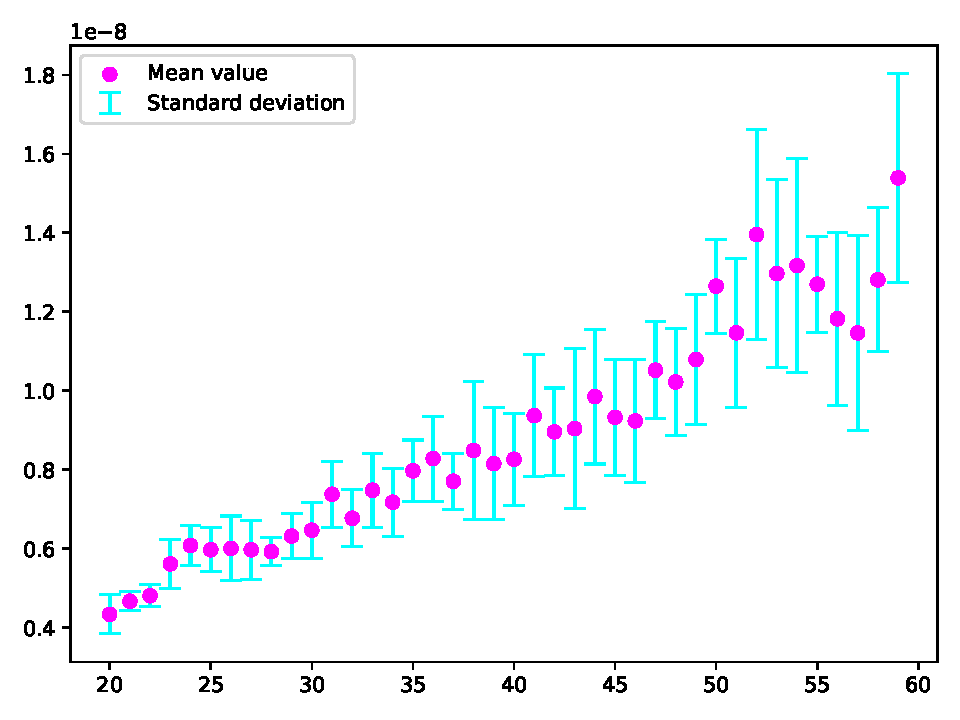
\includegraphics[width=\textwidth]{figures/n/cyclic_function_of_n_n_20_60__kappa_300}
        \caption{Cyclic.}\label{fig:nd}
    \end{subfigure}
    \caption{Plot of \(\text{avg}(\text{time}/(m \min(d, 1/\varepsilon)\log(\kappa)/\varepsilon))\) as a function of \(n\), using various variations with \(\varepsilon = 10^{-4}\) and \(m = 175\). Matrices are generated according to the framework presented in \Cref{data_genaration}. Forall \(n \in \inte 20 60 \), we generate 10 matrices of size \(n\) and sparsity \(m\).}\label{fig:n}
\end{figure}

We can assess the convergence depicted in~\Cref{fig:n} by comparing it to the outcomes presented in~\Cref{theoritical}. As outlined in~\Cref{random_cyclic_thm}, our anticipation was a linear progression concerning \(n\) in~\Cref{fig:nb} and~\Cref{fig:nd}. Remarkably, this linear trend is observed, even though it was originally expected only in terms of expectation. Referring to~\Cref{greedy_thm}, an evolution in \(\mathcal O(n^2/m)\) is expected in~\Cref{fig:nc}, and this prediction aligns with the observed outcomes. These numerical results are indeed promising.\\

The final validation involves examining~\Cref{main_thm}, suggesting that~\Cref{fig:na} should remain constant. Contrary to this expectation, the figure does not exhibit constancy. However, the growth rate is noticeably lower compared to the other variants, and there appears to be a tendency for the curve to plateau as \(n\) increases which is encouraging.


\subsubsection{Complexity as a function of \(m\)}

In order to experimentally show the convergence speed of theorems presented in~\Cref{theoritical}, we fixed the parameters \(n\) and \(\varepsilon\) and let \(m\) in \(\inte 60 300 \). Each matrix is generated using an exponential distribution according to the scheme\footnote{Note that here \(\kappa\) is not fixed.} presented in~\Cref{data_genaration}. The~\Cref{fig:m} displays the results.

\begin{figure}[H]
    \centering
    \begin{subfigure}[b]{.24\textwidth}
        \centering
        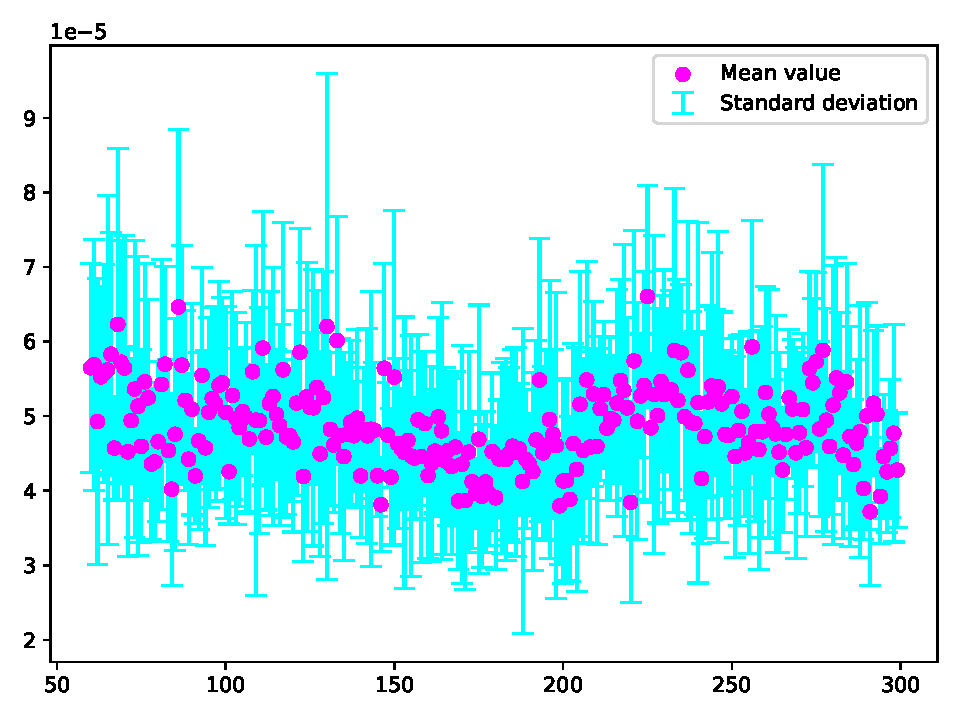
\includegraphics[width=\textwidth]{figures/m/random_function_of_m_n_10_m_20_90_kappa_524564.1271422369}
        \caption{Random.}\label{fig:ma}
    \end{subfigure}
    \hfill
    \begin{subfigure}[b]{.24\textwidth}
        \centering
        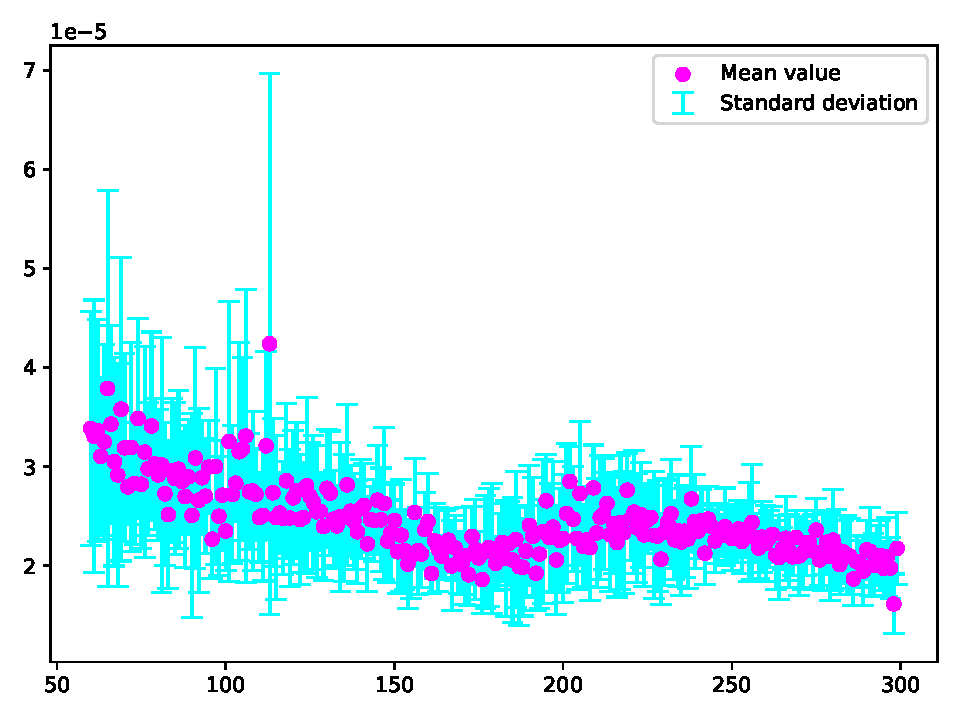
\includegraphics[width=\textwidth]{figures/m/random_cyclic_function_of_m_n_10_m_20_90_kappa_60194.24212737572}
        \caption{Random cyclic.}\label{fig:mb}
    \end{subfigure}
    \hfill
    \begin{subfigure}[b]{.24\textwidth}
        \centering
        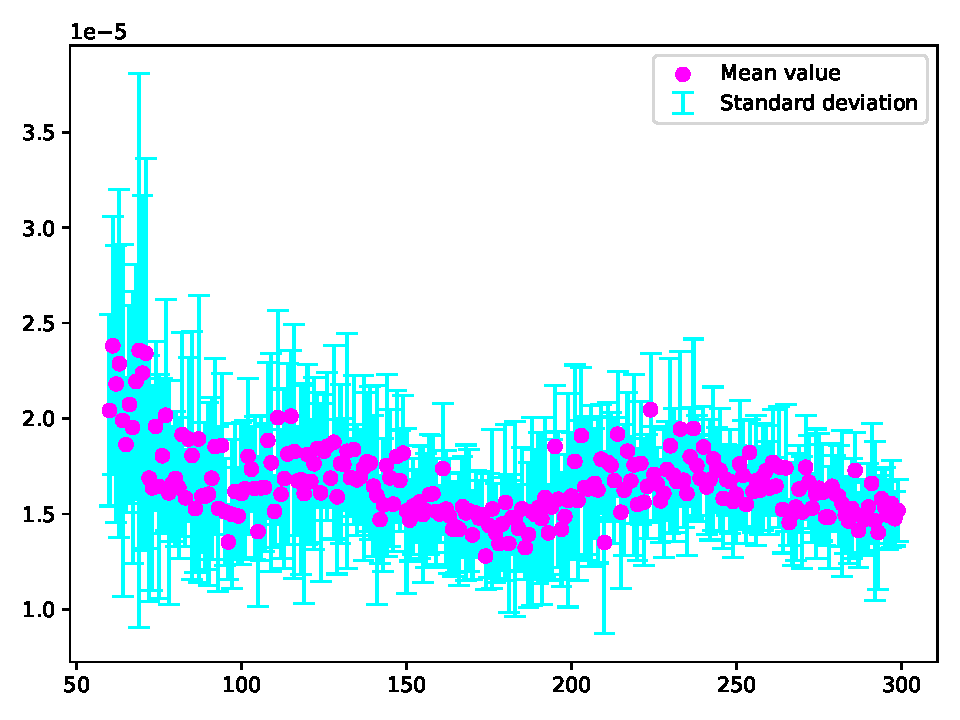
\includegraphics[width=\textwidth]{figures/m/greedy_function_of_m_n_10_m_20_90_kappa_241790.2230925089}
        \caption{Greedy.}\label{fig:mc}
    \end{subfigure}
    \hfill
    \begin{subfigure}[b]{.24\textwidth}
        \centering
        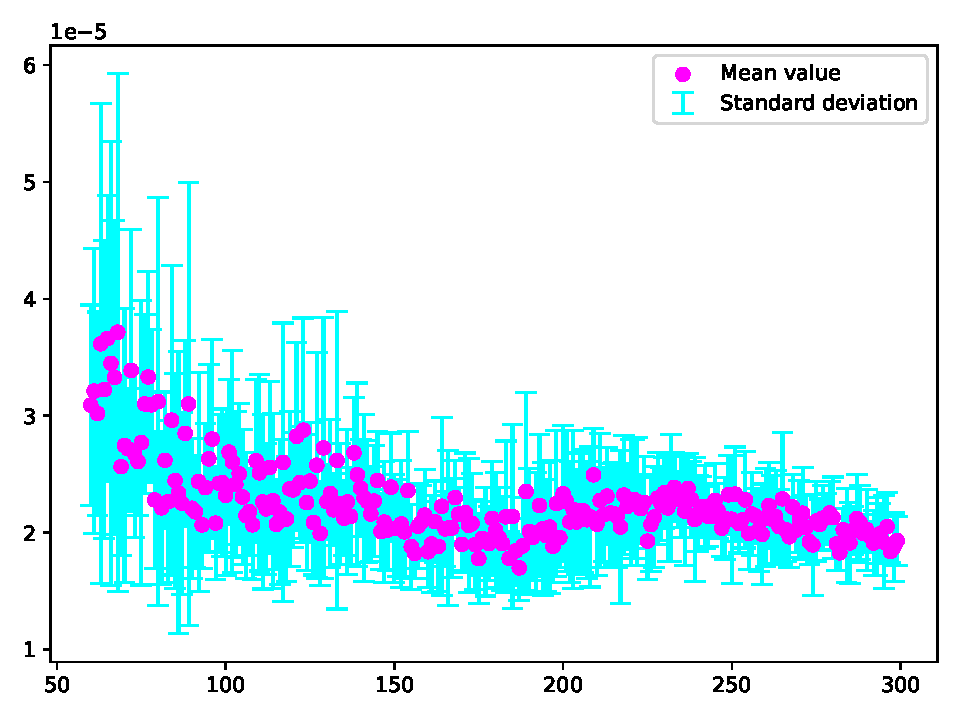
\includegraphics[width=\textwidth]{figures/m/cyclic_function_of_m_n_10_m_20_90_kappa_118817.63812510876}
        \caption{Cyclic.}\label{fig:md}
    \end{subfigure}
    \caption{Plot of \(\text{avg}(\text{time}/(\min(d, 1/\varepsilon)\log(\kappa)/\varepsilon))\) as a function of \(m\), using various variations with \(\varepsilon = 10^{-2}\) and \(n = 60\). Matrices are generated according to the framework presented in \Cref{data_genaration}. Forall \(m \in \inte 60 300 \), we generate 10 matrices of size \(n\) and sparsity \(m\).}\label{fig:m}
\end{figure}

Interpreting the plots in~\Cref{fig:m} using the theorems outlined in~\Cref{theoritical} poses challenges due to intrinsic connections between certain variables, such as \(d\) and \(m\) in the results. The expectation, based on~\Cref{greedy_thm}, is that the plot using the greedy \textsc{Osborn} method should remain flat, indicating no dependence on \(m\). However, contrary to this theoretical expectation, the observed plot does not exhibit this characteristic. A more nuanced understanding is provided by~\Cref{fig:m1}, where the relationship between~\Cref{fig:mc} and~\Cref{fig:m1a} suggests non-monotonic behavior.

\begin{figure}[H]
    \centering
    \begin{subfigure}[b]{.475\textwidth}
        \centering
        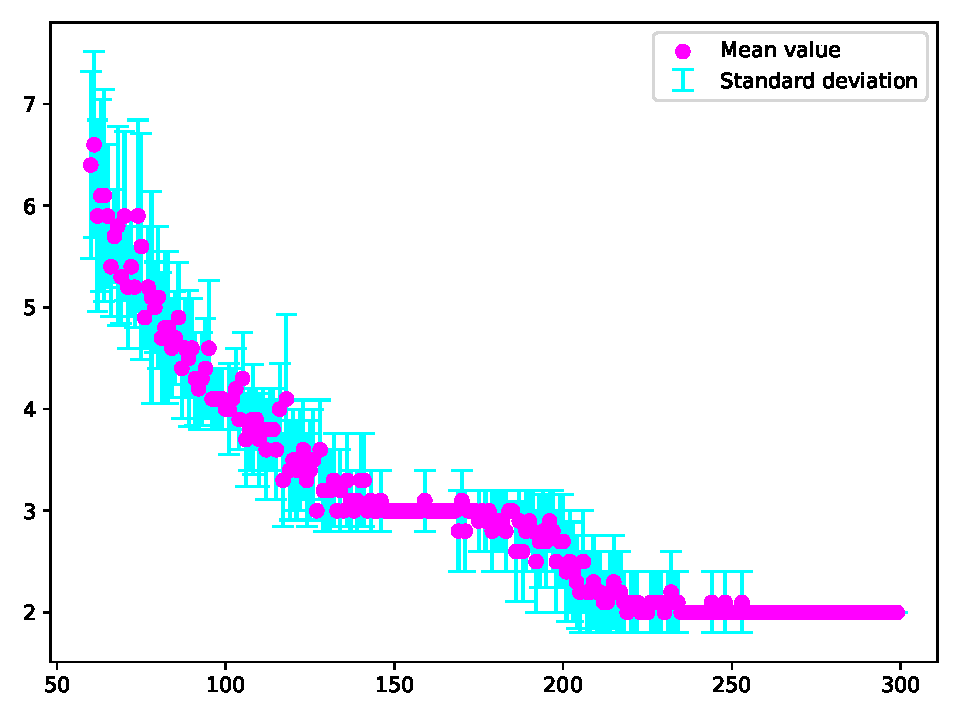
\includegraphics[width=.75\textwidth]{figures/m/d}
        \caption{Evolution of \(d\).}\label{fig:m1a}
    \end{subfigure}
    \hfill
    \begin{subfigure}[b]{.475\textwidth}
        \centering
        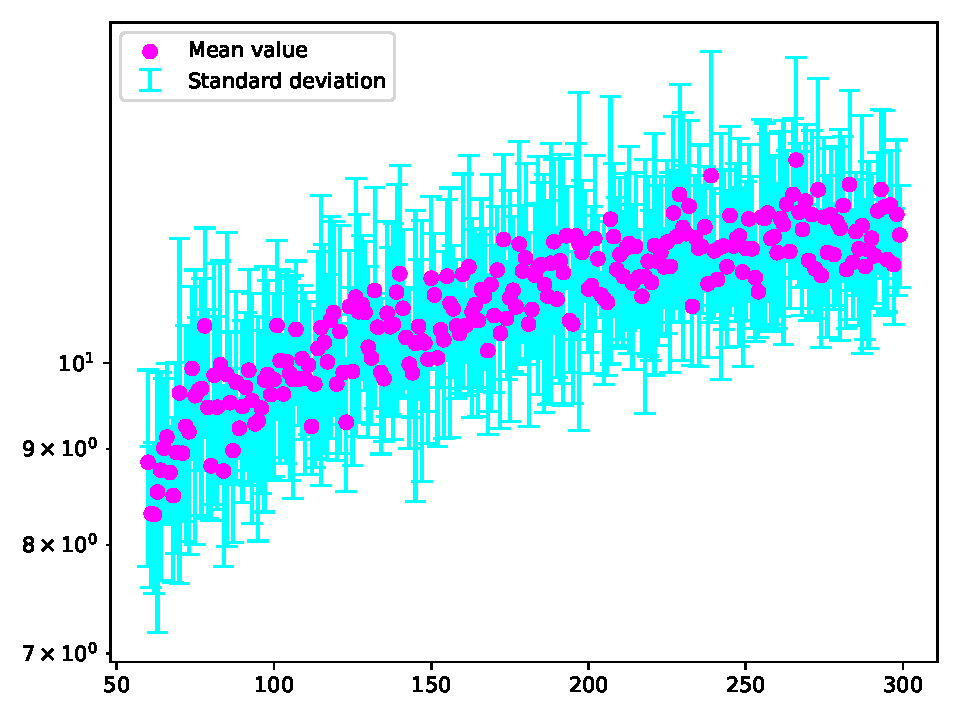
\includegraphics[width=.75\textwidth]{figures/m/kappa}
        \caption{Evolution of \(\log\kappa\).}\label{fig:m1b}
    \end{subfigure}
    \caption{Plots of \(\text{avg}(d)\) and \(\text{avg}(\log\kappa)\) as a function of \(m\), using \(n = 60\) and the framework presented in \Cref{data_genaration}. Forall \(m \in \inte 60 300 \), we generate 10 matrices of size \(n\) and sparsity \(m\).}\label{fig:m1}
\end{figure}

Specifically, as~\Cref{fig:m1a} decreases,~\Cref{fig:mc} increases, and vice versa, elucidating the non-monotonous trend observed. Additionally, insights from~\Cref{fig:m1b} contribute to an understanding of why the scaled time is decreasing overall for the greedy variant. Similar principles apply to the interpretation of the other plots. Notably, the random variant appears to be less affected by overall trends, suggesting a higher dependency on \(m\).\\

Unfortunately, the observed plots do not align with our expectations. They fail to exhibit a clear linear dependency for the three variants, contrary to the anticipated linear relationship.

\subsubsection{Complexity as a function of \(\kappa\)}

\subsubsection{Sparsity}

We conducted numerical experiments to investigate the behaviour of Osborn's algorithm in the presence of varying numbers of zero entries within randomly generated matrices. The goal is to experimentally see how tight the bounds provided in the article are.\\

% \begin{figure}[H]
%     \centering
%     \begin{subfigure}[b]{.32\textwidth}
%         \centering
%         \includegraphics[width=\textwidth]{figures/random_cyclic_n10,m_20_100_kappa_100}
%         \caption{\(\kappa=100\)}
%     \end{subfigure}
%     \hfill
%     \begin{subfigure}[b]{.32\textwidth}
%         \centering
%         \includegraphics[width=\textwidth]{figures/random_cyclic_n10,m_20_100_kappa_1000}
%         \caption{\(\kappa=10^3\)}
%     \end{subfigure}
%     \hfill
%     \begin{subfigure}[b]{.32\textwidth}
%         \centering
%         \includegraphics[width=\textwidth]{figures/random_cyclic_n10,m_20_100_kappa_1000000}
%         \caption{\(\kappa=10^6\)}
%     \end{subfigure}
%     \caption{Plot of \(\text{avg}(\text{time}/(n \min(d, 1/\varepsilon)\log(\kappa)/\varepsilon))\) as a function of \(m\), using the random cyclic variation with \(\varepsilon = 10^{-4}\). Matrices are generated according to the framework presented in \Cref{data_genaration}. For \(n = 10\) and values of \(m\) in \(\inte 20  {n} \), we generate 100 matrices of size \(n\) and sparsity \(m\) for different fixed values of \(\kappa\).}
% \end{figure}

% \begin{figure}[H]
%     \centering
%     \begin{subfigure}[b]{.32\textwidth}
%         \centering
%         \includegraphics[width=\textwidth]{figures/random_n10_m_20_100_kappa_100.pdf}
%         \caption{\(\kappa=100\)}
%     \end{subfigure}
%     \hfill
%     \begin{subfigure}[b]{.32\textwidth}
%         \centering
%         \includegraphics[width=\textwidth]{figures/random_n10_m_20_100_kappa_1000.0.pdf}
%         \caption{\(\kappa=10^3\)}
%     \end{subfigure}
%     \hfill
%     \begin{subfigure}[b]{.32\textwidth}
%         \centering
%         \includegraphics[width=\textwidth]{figures/random_n10_m_20_100_kappa_1000000.0.pdf}
%         \caption{\(\kappa=10^6\)}
%     \end{subfigure}
%     \caption{Plot of \(\text{avg}(\text{time}/(\min(d, 1/\varepsilon)\log(\kappa)/\varepsilon))\) as a function of \(m\), using the random variation with \(\varepsilon = 10^{-4}\). Matrices are generated according to the framework presented in \Cref{data_genaration}. For \(n = 10\) and values of \(m\) in \(\inte 20  {n} \), we generate 100 matrices of size \(n\) and sparsity \(m\) for different fixed values of \(\kappa\).}
% \end{figure}



\todo[inline, caption={Link with convex opti}]{Use obeservation 2.5 to compare with other convex optim algorithms.}

\todo[inline, caption={Per iteration}]{Look at per iteration runtime (5.2)}

\section{Conclusion and perspective}

Summary of the result obtained: pros and cons (limitation, problems, error in the articles, etc)
Possible improvement/extension 

\section{Connexion with the course}

MANDATORY SECTION:. What are the notions/results/algorithms presented in the course that are used or related to the one presented in this paper?

\listoftodos{}

\newpage
\printbibliography[heading=bibintoc]

\end{document}